

%!TEX root = ../thesis.tex
%******************************************************************************
\chapter[Conceptual Framework]{A Conceptual Framework for Feedback-Controlled Bulk Data Processing Systems}\label{ch:conceptual_framework}

%******************************************************************************

\section{Introduction} 

\begin{itemize}
	\item The concept for an adaptive Middleware for bulk data processing presented in chapter \ref{ch:adaptive_middleware} describes the ``What'' (what needs to be done) but not the ``How'' (how should it be done).
	\item The design, implementation and operation of such a system differs from common approaches to implement enterprise systems (what are these differences?)
	\begin{itemize}
		\item Design: Defining Service interfaces, defining aggregation rules, defining transports, defining integration architecture
		\item Implementation: Service implementation, Service Optimisation
		\item Operation: controller tuning, monitoring
	\end{itemize}
	\item In order to guide the implementation of an adaptive system for bulk data processing, a conceptual framework is needed
	\item It defines views, roles and tasks and their dependencies to describe the necessary steps for design, implementation and operation of system describe in Chapter \ref{ch:adaptive_middleware}.
	\item The conceptual model can be tailored to specific projects requirements, it does not have to be followed strictly.
\end{itemize}

\begin{figure}
	[htpb] \centering 
	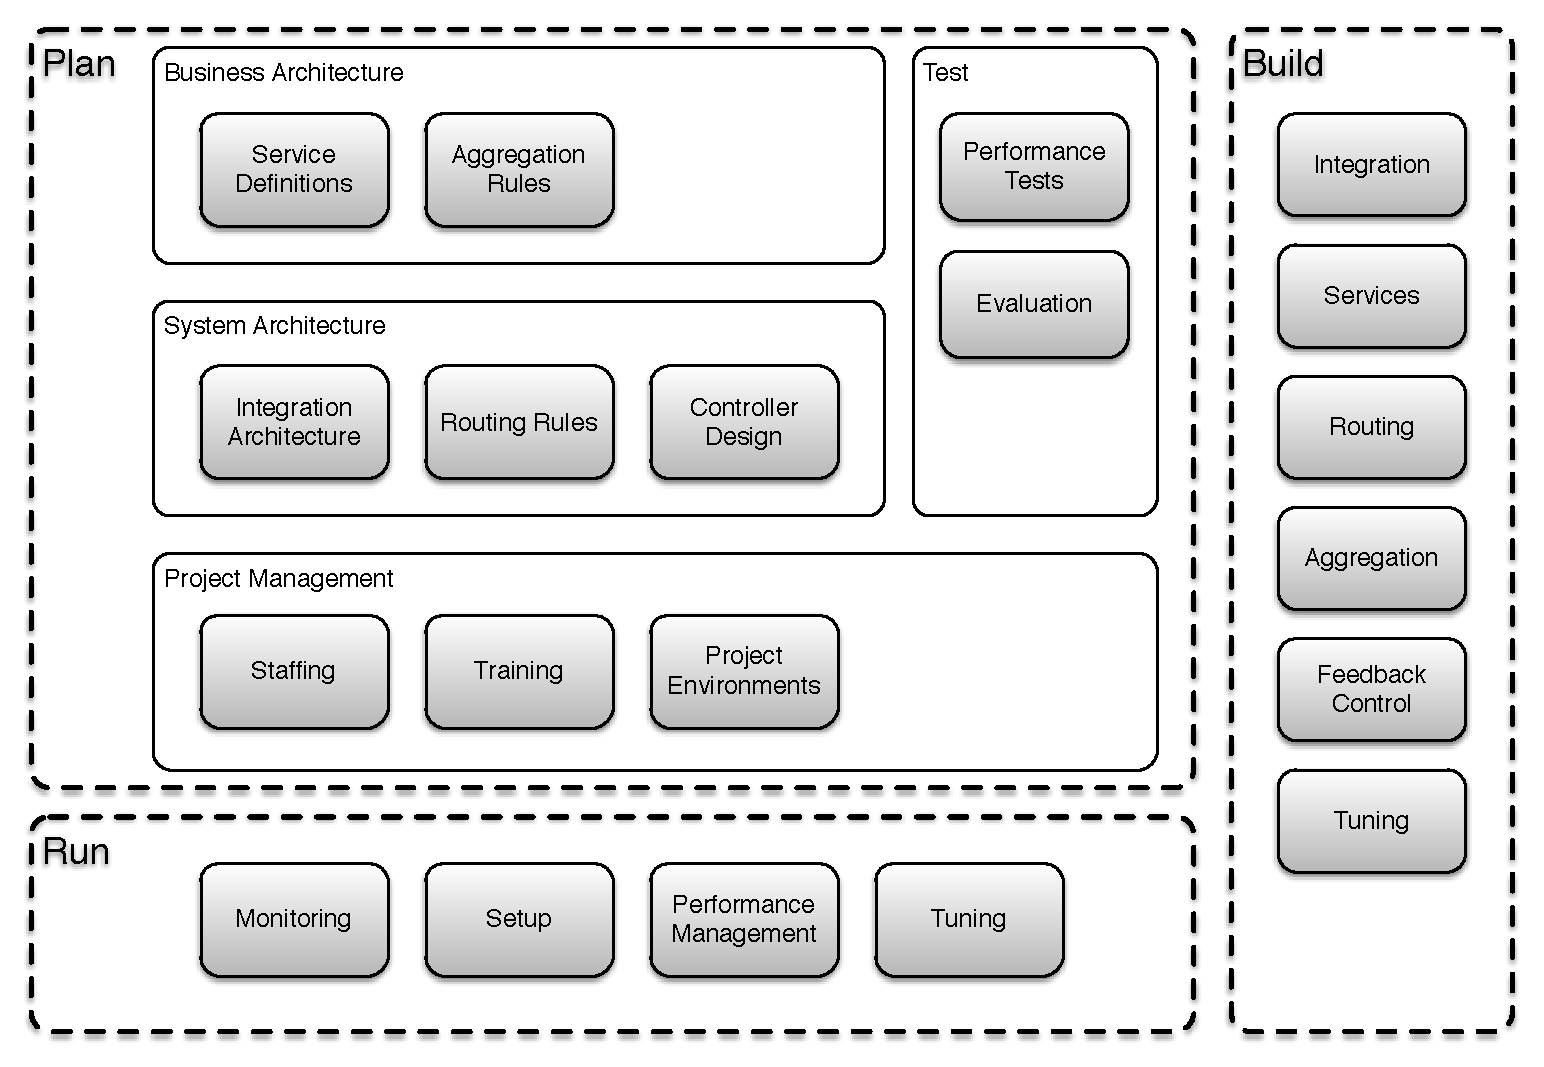
\includegraphics[width=\textwidth]{ch6_overview} \caption{Overview of Conceptual Framework} \label{fig:ch6_overview} 
\end{figure}

\section{Metamodel} 
The conceptual framework consists of the following entities:
\begin{itemize}
	\item View
	\begin{itemize}
		\item contains Tasks
	\end{itemize}
	\item Role
	\begin{itemize}
		\item processes Tasks
	\end{itemize}
	\item Task
	\begin{itemize}
		\item is contained in a View
		\item is processed by a Role
		\item produces Artifacts
		\item uses Tools
	\end{itemize}
	\item Deliverable
	\begin{itemize}
		\item is produced by a Task
	\end{itemize}
	\item Tool
	\begin{itemize}
		\item is used by a Task
	\end{itemize}
\end{itemize}

\begin{figure}
	[htpb] \centering 
	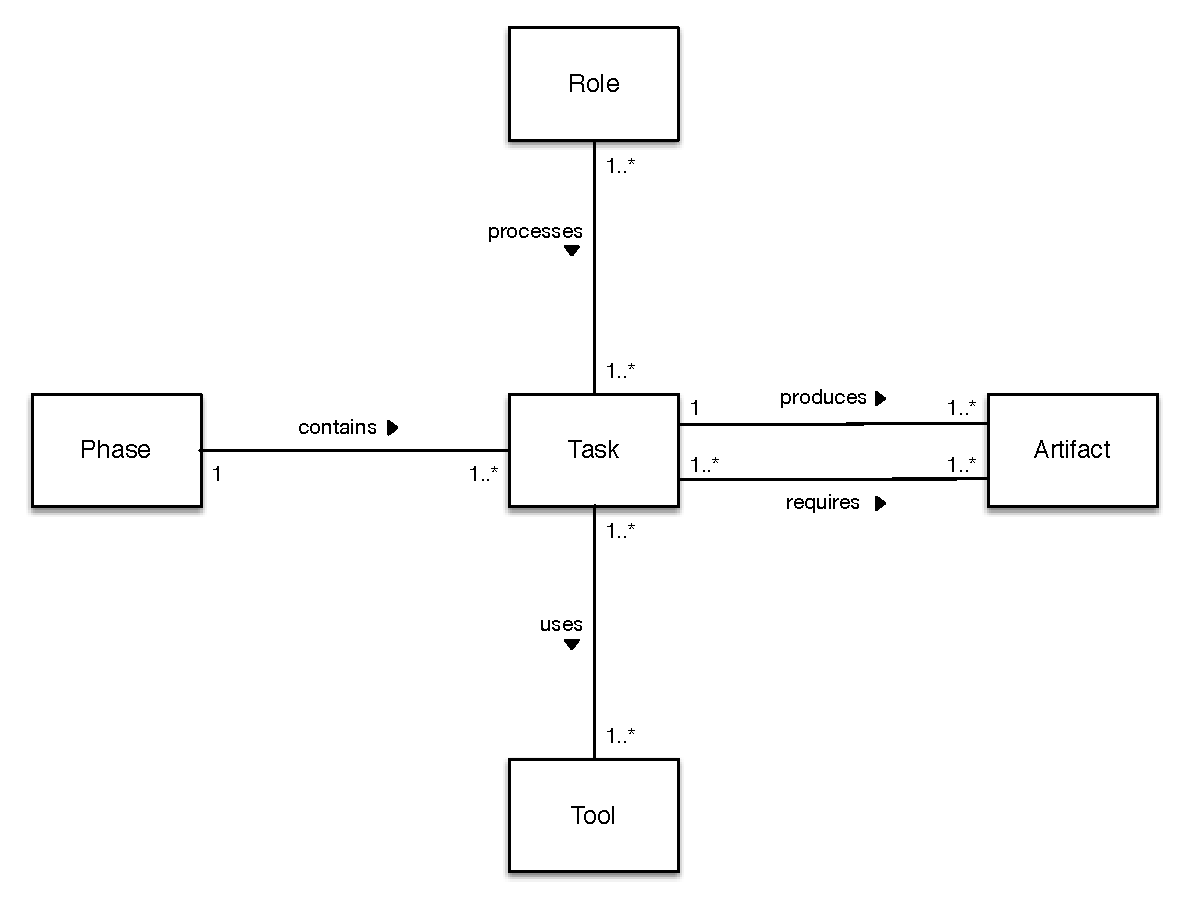
\includegraphics[width=\textwidth]{ch6_metamodel} 
	\caption{Metamodel} 
	\label{fig:ch6_metamodel} 
\end{figure}

\section{Phase}

\begin{itemize}
	\item Phases are the toplevel building blocks
	\item The framework defines the following phases
	\begin{itemize}
		\item Plan
		\item Build
		\item Run
	\end{itemize}
	\item Phases are aligned to phases commonly used by other software development frameworks and methodologies (examples?)
	\item It should be noted that the framework defines no requirements regarding the general order or mode in which theses phases should be processed. It is therefore possible to use this framework with different software development methodologies such as the Waterfall model, Scrum or the V-Modell.
\end{itemize}

\subsection{Plan}
\begin{minipage}{\textwidth}
	\captionof{table}{Phase: Plan}\label{table:ch6_View_Plan}
	\begin{tabular}
		{|m{2cm}|m{10cm}|} \hline \bfseries Phase & Plan\\
		\hline \bfseries Description & This phase contains tasks concerning the technical and business design of the system.\\
		\hline \bfseries Tasks & 
		\begin{itemize}
			\item Define System Architecture
			\item Define Integration Architecture
			\item Define Controller Architecture
			\item Define Service Interfaces
			\item Define Aggregation Rules
			\item Define Performance Tests
			\item Define Training Concept
		\end{itemize}
		\\
		\hline \bfseries Roles &
		\begin{itemize}
			\item Project Manager
			\item Business Analyst
			\item System Architect
			\item Service Architect
		\end{itemize}
		\\
		\hline 
	\end{tabular}
\end{minipage}

\subsection{Build}
\begin{minipage}{\textwidth}
\captionof{table}{Phase: Build}\label{table:ch6_View_Build}
\begin{tabular}
	{|m{2cm}|m{10cm}|} \hline \bfseries Phase & Build\\
	\hline \bfseries Description & This phase contains tasks concerning the implementation of the system.\\
	\hline \bfseries Tasks & 
	\begin{itemize}
		\item Implement Controller and Feedback Loop
		\item Implement Services
		\item Implement Aggregation Rules
		\item Perform Controller Tuning
	\end{itemize}
	\\
	\hline \bfseries Roles &
	\begin{itemize}
		\item Developer
		\item Service Developer
		\item System Architect
		\item Tester
	\end{itemize}
	\\
	\hline 
\end{tabular}
\end{minipage}

\subsection{Run}
\begin{minipage}{\textwidth}
\captionof{table}{Phase: Run}\label{table:ch6_View_Run}
\begin{tabular}
	{|m{2cm}|m{10cm}|} \hline \bfseries Phase & Run\\
	\hline \bfseries Description & This phase contains tasks concerning the operation of the implemented system in the production environment. \\
	\hline \bfseries Tasks & 
	\begin{itemize}
		\item Setup Monitoring infrastructure
		\item Setup Test and Integration Environment
		\item Deploy to Test and Integration Environment
		\item Perform Performance Tests
		\item Evaluate Performance Test Results
	\end{itemize}
	\\
	\hline \bfseries Roles &
	\begin{itemize}
		\item Operations Engineer
		\item Systems Architect
		\item Developer
	\end{itemize}
	\\
	\hline 
\end{tabular}
\end{minipage}

\section{Roles} 

\begin{itemize}
	\item Roles describe responsibilities and skills
	\item Roles are not the same as persons, a person can fulfill multiple roles at the same time
\end{itemize}

The following Roles are defined:
\begin{itemize}
	\item System Architect 
	\item Business Architect
	\item Developer
	\item Test Engineer
	\item Project Manager
	\item Operations Engineer 
	\item Service Architect 
	\item Service Developer
\end{itemize}

\subsection{System Architect} 
\begin{minipage}{\textwidth}
\captionof{table}{System Architect}\label{table:ch6_Role_System_Architect}
\begin{tabular}
	{|m{2cm}|m{10cm}|} \hline \bfseries Role & System Architect\\
	\hline \bfseries Description & The System Architect is responsible for designing the technical architecture of the system, including the integration and controller architecture.\\
	\hline \bfseries Tasks & 
	\begin{itemize}
		\item Define System Architecture 
		\item Define Integration Architecture
		\item Define Controller Architecture
		\item Define Service Interfaces (?)
	\end{itemize}
	\\
	\hline 
\end{tabular}
\end{minipage}

\subsection{Business Analyst}
\begin{minipage}{\textwidth}
\captionof{table}{Business Architect} \label{table:ch6_Role_Business_Analysist}
\begin{tabular}
	{|m{2cm}|m{10cm}|} \hline \bfseries Role & Business Analyst\\
	\hline \bfseries Description & The Business Architect is responsible for designing the business architecture of the system, including the definition of services and aggregation rules.\\
	\hline \bfseries Tasks & 
	\begin{itemize}
		\item Define Services (?)
		\item Define Aggregation Rules
	\end{itemize}
	\\
	\hline 
\end{tabular}
\end{minipage}

\subsection{Developer}
\begin{minipage}{\textwidth}
\captionof{table}{Developer} \label{table:ch6_Role_Developer}
\begin{tabular}
	{|m{2cm}|m{10cm}|} \hline \bfseries Role & Developer\\
	\hline \bfseries Description & The Developer is responsible for the implementation of the system, including the implementation and tuning of the feeback-controll loop.\\
	\hline \bfseries Tasks & 
	\begin{itemize}
		\item Implement Integration Mechanisms (?)
		\item Implement Aggregation Rules
		\item Implement Controller
		\item Perform Controller Tuning (?)
	\end{itemize}
	\\
	\hline 
\end{tabular}
\end{minipage}

\subsection{Tester}
\begin{minipage}{\textwidth}
\captionof{table}{Tester} \label{table:ch6_Role_Tester}
\begin{tabular}
	{|m{2cm}|m{10cm}|} \hline \bfseries Role & Test Engineer\\
	\hline \bfseries Description & The Tester is responsible for defining and performing the performance tests of the system.\\
	\hline \bfseries Tasks & 
	\begin{itemize}
		\item Define Performance Tests (?)
		\item Perform Performance Tests
	\end{itemize}
	\\
	\hline
\end{tabular}
\end{minipage}

\subsection{Project Manager}
\begin{minipage}{\textwidth}
\captionof{table}{Project Manager} \label{table:ch6_Role_Project_Manager}
\begin{tabular}
	{|m{2cm}|m{10cm}|} \hline \bfseries Role & Project Manager\\
	\hline \bfseries Description & The Project Manager is responsible for the project coordination, including the staffing and planing of the required environments.\\
	\hline \bfseries Tasks & 
	\begin{itemize}
		\item Plan Staffing (?)
		\item Plan Project Environments (Development / Testing / Integration / Production)
	\end{itemize}
	\\
	\hline 	
\end{tabular}
\end{minipage}

\subsection{Operations Engineer}
\begin{minipage}{\textwidth}
\captionof{table}{Operations Engineer} \label{table:ch6_Role_Operations_Engineer}
\begin{tabular}
	{|m{2cm}|m{10cm}|} \hline \bfseries Role & Operations Engineer\\
	\hline \bfseries Description & The Operations Engineer is responsible for operating the system, including setup, deployment and monitoring.\\
	\hline \bfseries Tasks & 
	\begin{itemize}
		\item Setup Monitoring Infrastructure
		\item Setup Test and Integration Environment
		\item Deploy to Test and Integration Environment 
	\end{itemize}
	\\
	\hline 
\end{tabular}
\end{minipage}

\subsection{Service Architect}
\begin{minipage}{\textwidth}
\captionof{table}{Service Architect} \label{table:ch6_Role_Service_Architect}
\begin{tabular}
	{|m{2cm}|m{10cm}|} \hline \bfseries Role & Service Architect\\
	\hline \bfseries Description & The Service Architect is responsible for designing the technical architecture of services.\\
	\hline \bfseries Tasks & 
	\begin{itemize}
		\item Define Service Interfaces
	\end{itemize}
	\\
	\hline 
\end{tabular}
\end{minipage}

\subsection{Service Developer}
\begin{minipage}{\textwidth}
\captionof{table}{Service Developer} \label{table:ch6_Role_Service_Developer}
\begin{tabular}
	{|m{2cm}|m{10cm}|} \hline \bfseries Role & Service Developer\\
	\hline \bfseries Description & The Service Developer is responsible for implementing the services.\\
	\hline \bfseries Tasks & 
	\begin{itemize}
		\item Implement Service Interface
	\end{itemize}
	\\
	\hline 
\end{tabular}
\end{minipage}

\section{Tasks}
\label{sec:ch6_tasks}

\begin{itemize}
	\item Main entities of the conceptual framework, define what should be done.
	\item Tasks depend on each other, some tasks must be processed in a certain order
\end{itemize}

\begin{figure}[htpb] \centering 
	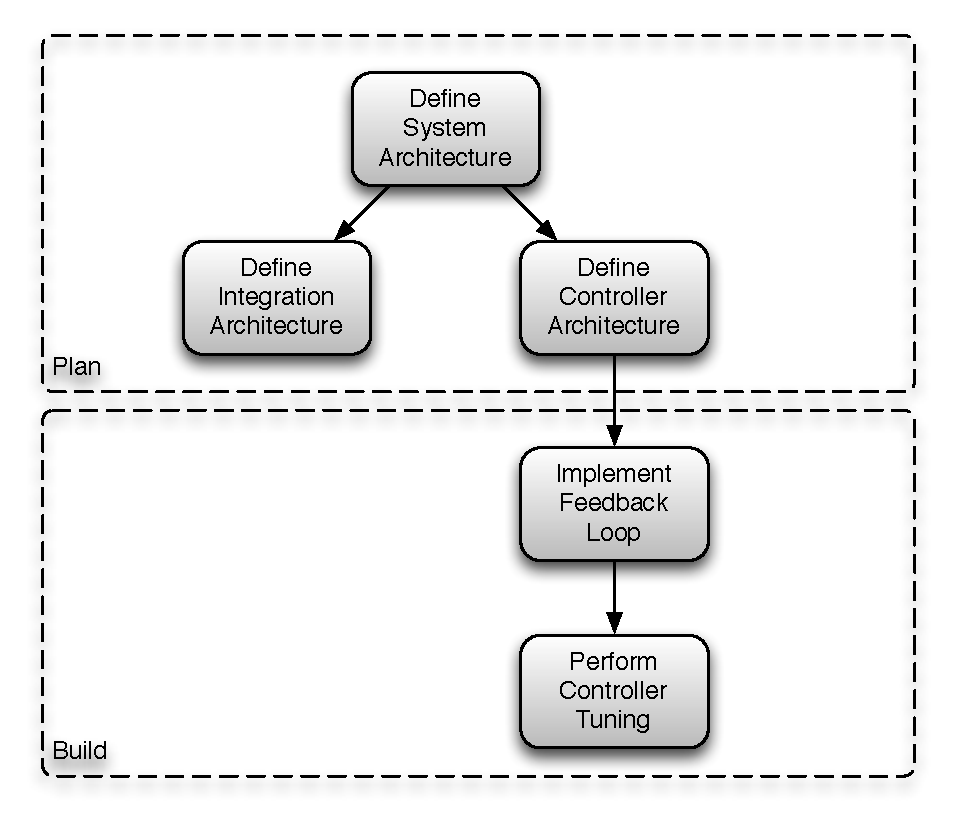
\includegraphics[width=\textwidth]{ch6_dependencies} 
	\caption{Tasks depend on each other} 
	\label{fig:ch6_dependencies} 
\end{figure}

\begin{itemize}
	\item Define Business Architecture
	\begin{itemize}
		\item Define Service Interfaces
		\item Define Aggregation Rules
	\end{itemize}
	\item Define System Architecture 
	\begin{itemize}
		\item Define Integration Architecture
		\begin{itemize}
			\item Transports
			\item Distribution
		\end{itemize}
		\item Define Routing Rules
		\item Define Controller Architecture 
		\begin{itemize}
			\item Define Control Problem 
			\item Define Input/Output Variables 
		\end{itemize}
		\item Define Routing Rules
	\end{itemize}
	\item Implement Controller / Feedback Loop
	\item Perform Controller Tuning 
	\begin{itemize}
		\item System Model/System Identification 
		\item Static Tests
		\item Step Tests
	\end{itemize}
	\item Implement Integration Architecture
	\item Implement Service Interfaces
	\item Implement Aggregation Rules 
	\item Implement Routing Rules
	\item Define Performance Tests 
	\item Setup Monitoring infrastructure
	\item Setup Test and Integration Environment
	\item Perform Performance Tests
	\item Evaluate Performance Test Results
	\item Define Training Concept
	\item Staffing
\end{itemize}

\subsection{Define Business Architecture}

\begin{itemize}
	\item The business architecture defines the business components of the system and their relationships independantly of the technical implementation.
	\item Except from the described subtasks, the task is not specific to the conceptual model.
\end{itemize}

\subsection{Define Service Interfaces}
\begin{minipage}{\textwidth}
\captionof{table}{Define Service Interfaces} \label{table:ch6_Task_Define_Service_Interfaces}
\begin{tabular}
	{|m{3cm}|m{10cm}|} \hline \bfseries What & Define Service Interfaces\\
	\hline \bfseries Why & Lorem ipsum\\
	\hline \bfseries Who & Business Architect\\
	\hline \bfseries Artifacts & Service Interface Definitions\\
	\hline \bfseries Challenges & Lorem Ipsum\\
	\hline 
\end{tabular}
\end{minipage}

\begin{itemize}
	\item Definition of service operations, every service needs operations for single event and batch processing
	\begin{itemize}
		\item Distinct operations for batch and single event processing
		\item common operation for both processing styles (list interface)
	\end{itemize}
	\item Defines functional format of input and output data
	\item Does not include informations about the technical format, such as \ac{XML} or \ac{JSON}, and the integration style, such SOAP or \ac{REST}
\end{itemize}

\subsection{Define Aggregation Rules}
\begin{minipage}{\textwidth}
\captionof{table}{Define Aggregation Rules} \label{table:ch6_Task_Define_Aggregation_Rules}
\begin{tabular}
	{|m{3cm}|m{10cm}|} \hline \bfseries What & Define Aggregation Rules\\
	\hline \bfseries Why & Lorem ipsum\\
	\hline \bfseries Who & Business Architect\\
	\hline \bfseries Artifacts & Aggregation Rules\\
	\hline \bfseries Challenges & Lorem Ipsum\\
	\hline 
\end{tabular}
\end{minipage}

\begin{itemize}
	\item Definition of rules used in the aggregator for correlating events
	\item Different options
	\begin{itemize}
		\item No correlation
		\begin{itemize}
			\item Simple solution
			\item even distribution of events
			\item optimization is not or hardly possible
		\end{itemize}
		\item Business correlation
		\begin{itemize}
			\item analysation of processed data needed
			\item no even distribution of data (depending on correlation rule), leads to uneven distribution of latency
			\item optimization is possible
		\end{itemize}
		\item Technical correlation
		\begin{itemize}
			\item analysation of processed data needed
			\item Rules can be defined after integration architecture
			\item no even distribution of data (depending on correlation rule), leads to uneven distribution of latency
			\item optimization (?)
		\end{itemize}
	\end{itemize}
\end{itemize}

\subsection{Define System Architecture }
\begin{minipage}{\textwidth}
\captionof{table}{Define System Architecture} \label{table:ch6_Task_Define_System_Architecture}
\begin{tabular}
	{|m{3cm}|m{10cm}|} \hline \bfseries What & Define System Architecture
	Subtasks:
	\begin{itemize}
		\item Define Integration Architecture
		\item Define Controller Architecture
	\end{itemize}
	\\
	\hline \bfseries Why & The System Architecture defines the technical architecture of the system.\\
	\hline \bfseries Who & System Architect\\
	\hline \bfseries Input & 
		\begin{itemize}
			\item Business Architecture
			\item Service Interface Definitions
		\end{itemize}
	\\
	\hline \bfseries Output & System Architecture\\
	\hline \bfseries Tools & \ac{UML}\\
	\hline \bfseries Challenges & \\
	\hline 
\end{tabular}
\end{minipage}

\begin{itemize}
	\item Except from the described subtasks, the task is not specific to the conceptual model.
\end{itemize}

\subsection{Define Integration Architecture}
\begin{minipage}{\textwidth}
\captionof{table}{Define Integration Architecture} \label{table:ch6_Task_Define_Integration_Architecture}
\begin{tabular}
	{|m{3cm}|m{10cm}|} \hline \bfseries What & Define Integration Architecture\\
	\hline \bfseries Why & \\
	\hline \bfseries Who & System Architect\\
	\hline \bfseries Input & 
		\begin{itemize}
			\item Business Architecture
			\item Service Interface Definitions
		\end{itemize}
	\\
	\hline \bfseries Output & Integration Architecture\\
	\hline \bfseries Challenges & \\
	\hline 
\end{tabular}
\end{minipage}

\begin{itemize}
	\item Definition of integration architecture
	\begin{itemize}
		\item Sychronous, e.g. webservices
		\item Asynchronous, e.g. message queues
	\end{itemize}
	\item Definition of transports
	\begin{itemize}
		\item JMS
		\item SOAP
		\item REST
		\item FTP
		\item DB
	\end{itemize}
	\item Different transports / integration patterns needed for different aggregation sizes:
	\begin{itemize}
		\item Large messages should not be transferred over the messaging bus
		\item Options for large messages:
		\begin{itemize}
			\item File-based integration and transfer using FTP or database
			\item Message-Slip EIP pattern
		\end{itemize}
	\end{itemize}
\end{itemize}

\subsection{Define Routing Rules}

\begin{minipage}{\textwidth}
\captionof{table}{Define Routing Rules} \label{table:ch6_Task_Define_Routing_Rules}
\begin{tabular}
	{|m{3cm}|m{10cm}|} \hline \bfseries What & Define Routing Rules\\
	\hline \bfseries Why & \\
	\hline \bfseries Who & System Architect\\
	\hline \bfseries Input & 
		\begin{itemize}
			\item Integration Architecture
		\end{itemize}
	\\
	\hline \bfseries Output & Routing Rules Definition\\
	\hline \bfseries Challenges & Finding the data aggregation threshold to route messages to the appropriate service endpoint.\\
	\hline 
\end{tabular}
\end{minipage}

\begin{itemize}
	\item Depending on the size of the aggregated message, the Router routes the message to the appropriate service endpoint, which is either optimized for batch or single event processing.
	\item The routing rules define, which service endpoint should be called for a given aggregation size.
\end{itemize}

\subsection{Define Controller Architecture}
\begin{minipage}{\textwidth}
\captionof{table}{Define Controller Architecture} \label{table:ch6_Task_Define_Controller_Architecture}
\begin{tabular}
	{|m{3cm}|m{10cm}|} \hline \bfseries What & Define Controller Architecture\\
	\hline \bfseries Why & \\
	\hline \bfseries Who & System Architect\\
	\hline \bfseries Input & System Architecture\\
	\hline \bfseries Output & Controller Architecture\\
	\hline \bfseries Artifacts & System Architecture\\
	\hline \bfseries Challenges & \\
	\hline 
\end{tabular}
\end{minipage}

\begin{itemize}
	\item Design of the controller architecture implemented by the system
	\item For example
	\begin{itemize}
		\item PID Controller
		\item Fuzzy Controller
	\end{itemize}
	\item Depends on control problem and system dynamics (linear, non-linear)
\end{itemize}

\subsubsection{Define Control Problem}
\todo[inline]{Do we need this task or is this already fixed with the proposed middleware architecture?}
\begin{minipage}{\textwidth}
\captionof{table}{Define Control Problem} \label{table:ch6_Task_Define_Control_Problem}
\begin{tabular}
	{|m{3cm}|m{10cm}|} \hline \bfseries What & Define System Architecture\\
	\hline \bfseries Why & Lorem ipsum\\
	\hline \bfseries Who & System Architect\\
	\hline \bfseries Artifacts & System Architecture\\
	\hline \bfseries Challenges & Lorem Ipsum\\
	\hline \bfseries Best practises & Lorem ipsum\\
	\hline 
\end{tabular}
\end{minipage}

\subsubsection{Define Input/Output Variables}
\begin{minipage}{\textwidth}
\captionof{table}{Define Input/Output Variables} \label{table:ch6_Task_Define_Controller_Variables}
\begin{tabular}
	{|m{3cm}|m{10cm}|} \hline \bfseries What & Define Input/Output Variables\\
	\hline \bfseries Why & Lorem ipsum\\
	\hline \bfseries Who & System Architect\\
	\hline \bfseries Artifacts & System Architecture\\
	\hline \bfseries Challenges & Lorem Ipsum\\
	\hline \bfseries Best practises & Lorem ipsum\\
	\hline 
\end{tabular}
\end{minipage}

\begin{itemize}
	\item Definition of input and output variables of the controller
	\item for example
	\begin{itemize}
		\item Number of messages in the system
		\item Input queue length
		\item current end-to-end latency
		\item current throughput
	\end{itemize}
	\item selected input variables should be measured easily and directly, without delay such as when calculating averages
\end{itemize}

\subsection{Implement Controller}
\begin{minipage}{\textwidth}
\captionof{table}{Implement Controller / Feedback Loop} \label{table:ch6_Task_Implement_Controller}
\begin{tabular}
	{|m{3cm}|m{10cm}|} \hline \bfseries What & Implement Controller\\
	\hline \bfseries Why & Lorem ipsum\\
	\hline \bfseries Who & System Architect\\
	\hline \bfseries Input & Controller Architecture\\
	\hline \bfseries Artifacts & Controller Implementation\\
	\hline \bfseries Challenges & 
		\begin{itemize}
			\item Sensor performance
			\item Distributed sensors 
			\item Framework vs. custom development
		\end{itemize}\\
	\hline 
\end{tabular}
\end{minipage}

\begin{itemize}
	\item Implementation of Controller Architecture including
	\begin{itemize}
		\item Sensors
		\item Controller
		\item Actuator
	\end{itemize}
	\item Implement JMX Beans for monitoring purposes
\end{itemize}

\subsection{Perform Controller Tuning}
\subsubsection{System Model/System Identification}
\todo[inline]{Should this be a Sub-Task of Definition of Controller Architecture?}
\begin{minipage}{\textwidth}
	\captionof{table}{System Model/System Identification} \label{table:ch6_Task_Controler_Tuning} 
	\begin{tabular}
		{|m{3cm}|m{10cm}|} \hline \bfseries What & Define System Architecture\\
		\hline \bfseries Why & Lorem ipsum\\
		\hline \bfseries Who & System Architect\\
		\hline \bfseries Artifacts & System Architecture\\
		\hline \bfseries Challenges & Lorem Ipsum\\
		\hline 
	\end{tabular}
\end{minipage}

\subsubsection{Static Tests}
\begin{minipage}{\textwidth}
\captionof{table}{Static Tests} \label{table:ch6_Task_Static_Tests}
\begin{tabular}
	{|m{3cm}|m{10cm}|} \hline \bfseries What & Static Tests\\
	\hline \bfseries Why & Lorem ipsum\\
	\hline \bfseries Who & System Architect\\
	\hline \bfseries Artifacts & System Architecture\\
	\hline \bfseries Challenges & Lorem Ipsum\\
	\hline 
\end{tabular}
\end{minipage}

\subsubsection{Step Tests}
\begin{minipage}{\textwidth}
\captionof{table}{Step Tests} \label{table:ch6_Task_Step_Tests}
\begin{tabular}
	{|m{3cm}|m{10cm}|} \hline \bfseries What & Step Tests\\
	\hline \bfseries Why & Lorem ipsum\\
	\hline \bfseries Who & System Architect\\
	\hline \bfseries Artifacts & System Architecture\\
	\hline \bfseries Challenges & Lorem Ipsum\\
	\hline 
\end{tabular}
\end{minipage}

\subsection{Implement Service Interfaces / Test / Deploy}
\begin{minipage}{\textwidth}
\captionof{table}{Implement Service Interfaces} \label{table:ch6_Task_Implement_Service_Interfaces}
\begin{tabular}
	{|m{3cm}|m{10cm}|} \hline \bfseries What & Implement Service Interfaces\\
	\hline \bfseries Why & Lorem ipsum\\
	\hline \bfseries Who & System Architect\\
	\hline \bfseries Input & Service Interface Definitions\\
	\hline \bfseries Artifacts & System Architecture\\
	\hline \bfseries Challenges & Lorem Ipsum\\
	\hline 
\end{tabular}
\end{minipage}

\begin{itemize}
	\item Implementation of business services
	\item Batch implementation / single event implementation
	\item Batch optimisation
\end{itemize}

\subsection{Implement Aggregation Rules}
\begin{minipage}{\textwidth}
\captionof{table}{Implement Aggregation Rules} \label{table:ch6_Task_Implement_Aggregation_Rules}
\begin{tabular}
	{|m{3cm}|m{10cm}|} \hline \bfseries What & Implement Aggregation Rules\\
	\hline \bfseries Why & Lorem ipsum\\
	\hline \bfseries Who & System Architect\\
	\hline \bfseries Input & Aggregation Rules\\
	\hline \bfseries Artifacts & System Architecture\\
	\hline \bfseries Challenges & Lorem Ipsum\\
	\hline 
\end{tabular}
\end{minipage}

\begin{itemize}
	\item Implementation of aggregation rules
	\item Rules should be configurable during run-time or configuration-time. Should not be hard-coded.
\end{itemize}

\subsection{Define Performance Tests}
\begin{minipage}{\textwidth}
\captionof{table}{Define Performance Tests} \label{table:ch6_Task_Define_Performance_Tests}
\begin{tabular}
	{|m{3cm}|m{10cm}|} \hline \bfseries What & Define Performance Tests\\
	\hline \bfseries Why & Lorem ipsum\\
	\hline \bfseries Who & System Architect\\
	\hline \bfseries Artifacts & System Architecture\\
	\hline \bfseries Challenges & Lorem Ipsum\\
	\hline 
\end{tabular}
\end{minipage}

\begin{itemize}
	\item Define load scenarios
	\item define test data
	\item Implement event generator
	\item Implementation of tools/scripts for evaluation and data visualisation
\end{itemize}

\subsection{Setup Monitoring infrastructure}
\begin{minipage}{\textwidth}
\captionof{table}{Setup Monitoring infrastructure} \label{table:ch6_Task_Setup_Monitoring_infrastructure}
\begin{tabular}
	{|m{3cm}|m{10cm}|} \hline \bfseries What & Setup Monitoring infrastructuree\\
	\hline \bfseries Why & Lorem ipsum\\
	\hline \bfseries Who & System Architect\\
	\hline \bfseries Artifacts & System Architecture\\
	\hline \bfseries Challenges & Lorem Ipsum\\
	\hline 
\end{tabular}
\end{minipage}

\begin{itemize}
	\item Integrate jmx services into monitoring infrastracture
\end{itemize}

\subsection{Setup Test and Integration Environment}
\begin{minipage}{\textwidth}
\captionof{table}{Setup Test and Integration Environment} \label{table:ch6_Task_Setup_Test_Environment}
\begin{tabular}
	{|m{3cm}|m{10cm}|} \hline \bfseries What & Setup Test and Integration Environment\\
	\hline \bfseries Why & Lorem ipsum\\
	\hline \bfseries Who & System Architect\\
	\hline \bfseries Artifacts & System Architecture\\
	\hline \bfseries Challenges & Lorem Ipsum\\
	\hline 
\end{tabular}
\end{minipage}

\begin{itemize}
	\item Setup / Mock external Services
	\item setup test data
	\item Deployment
\end{itemize}

\subsection{Perform Performance Tests}
\begin{minipage}{\textwidth}
\captionof{table}{Perform Performance Tests} \label{table:ch6_Task_Perform_Performance_Tests}
\begin{tabular}
	{|m{3cm}|m{10cm}|} \hline \bfseries What & Perform Performance Tests\\
	\hline \bfseries Why & Lorem ipsum\\
	\hline \bfseries Who & System Architect\\
	\hline \bfseries Artifacts & System Architecture\\
	\hline \bfseries Challenges & Lorem Ipsum\\
	\hline 
\end{tabular}
\end{minipage}

\subsection{Evaluate Performance Test Results}
\begin{minipage}{\textwidth}
\captionof{table}{Evaluate Performance Test Results} \label{table:ch6_Evaluate_Performance_Results}
\begin{tabular}
	{|m{3cm}|m{10cm}|} \hline \bfseries What & Evaluate Performance Test Results\\
	\hline \bfseries Why & Lorem ipsum\\
	\hline \bfseries Who & System Architect\\
	\hline \bfseries Artifacts & System Architecture\\
	\hline \bfseries Challenges & Lorem Ipsum\\
	\hline 
\end{tabular}
\end{minipage}

\begin{itemize}
	\item Visualise the test results using the tools/skripts implemented in task Define Performance Tests.
\end{itemize}

\subsection{Define Training Concept}
\begin{minipage}{\textwidth}
\captionof{table}{Define Training Concept} \label{table:ch6_Task_Define_Training_Concept}
\begin{tabular}
	{|m{3cm}|m{10cm}|} \hline \bfseries What & Define Training Concept\\
	\hline \bfseries Why & Lorem ipsum\\
	\hline \bfseries Who & System Architect\\
	\hline \bfseries Artifacts & System Architecture\\
	\hline \bfseries Challenges & Lorem Ipsum\\
	\hline 
\end{tabular}
\end{minipage}

\begin{itemize}
	\item define target audience, e.g. operations engineer
	\item define training content
	\begin{itemize}
		\item Different operation modes (batch, single event processing)
		\item performance characteristics (regarding latency and throughput) depend on current operation mode
		\item Tuning options (Controller, Aggregation Rules, Routing Rules)
	\end{itemize}
\end{itemize}

\subsection{Staffing}
\begin{minipage}{\textwidth}
\captionof{table}{Staffing} \label{table:ch6_Task_Staffing}
\begin{tabular}
	{|m{3cm}|m{10cm}|} \hline \bfseries What & Staffing\\
	\hline \bfseries Why & Lorem ipsum\\
	\hline \bfseries Who & Project Manager\\
	\hline \bfseries Artifacts & Staffing Plan\\
	\hline \bfseries Challenges & Lorem Ipsum\\
	\hline 
\end{tabular}
\end{minipage}

\begin{itemize}
	\item Special skills needed for staffing the project
	\item Adaptive Middleware concepts
	\item System Architect:
	\begin{itemize}
		\item Controller Design
	\end{itemize}
	\item Software Engineer:
	\begin{itemize}
		\item Controller Implementation and Tuning
	\end{itemize}
\end{itemize}

\section{Artifacts}

\begin{itemize}
	\item An Artifact is a result of a task
	\item Additionally, an artifact can be a prerequisite of a task
\end{itemize}

\begin{itemize}
	\item Business Architecture
	\item Service Interface Definition
	\item Aggregation Rules
	\item System Architecture
	\item Integration Architecture
	\item Routing Rules
	\item Controller Architecture
	\item System Model
	\item Performance Test Concept
	\item Training Concept
\end{itemize}

\subsection{Business Architecture}
\begin{minipage}{\textwidth}
\captionof{table}{Business Architecture} \label{table:ch6_Artifact_Business_Architecture}
\begin{tabular}
	{|m{2cm}|m{10cm}|} \hline \bfseries Artifact & Business Architecture\\
	\hline \bfseries Description & Lorem ipsum\\
	\hline \bfseries Task & 
	\begin{itemize}
		\item Define Business Architecture 
	\end{itemize}
	\\
	\hline \bfseries Role & Business Architect\\
	\hline 
\end{tabular}
\end{minipage}

\subsection{Service Interface Definition}
\begin{minipage}{\textwidth}
\captionof{table}{Business Architecture} \label{table:ch6_Artifact_Service_Interface_Definition}
\begin{tabular}
	{|m{2cm}|m{10cm}|} \hline \bfseries Artifact & Business Architecture\\
	\hline \bfseries Description & Lorem ipsum\\
	\hline \bfseries Task & 
	\begin{itemize}
		\item Define Business Architecture 
	\end{itemize}
	\\
	\hline \bfseries Role & Business Architect\\
	\hline 
\end{tabular}
\end{minipage}

\subsection{Aggregation Rules}
\begin{minipage}{\textwidth}
\captionof{table}{Business Architecture} \label{table:ch6_Artifact_Aggregation_Rules}
\begin{tabular}
	{|m{2cm}|m{10cm}|} \hline \bfseries Artifact & Business Architecture\\
	\hline \bfseries Description & Lorem ipsum\\
	\hline \bfseries Task & 
	\begin{itemize}
		\item Define Business Architecture 
	\end{itemize}
	\\
	\hline \bfseries Role & Business Architect\\
	\hline 
\end{tabular}
\end{minipage}

\subsection{System Architecture}
\begin{minipage}{\textwidth}
\captionof{table}{System Architecture} \label{table:ch6_Artifact_System_Architecture}
\begin{tabular}
	{|m{2cm}|m{10cm}|} \hline \bfseries Artifact & System Architecture\\
	\hline \bfseries Description & Lorem ipsum\\
	\hline \bfseries Task & 
	\begin{itemize}
		\item Define System Architecture 
	\end{itemize}
	\\
	\hline \bfseries Role & System Architect\\
	\hline 
\end{tabular}
\end{minipage}

\subsection{Integration Architecture}
\begin{minipage}{\textwidth}
\captionof{table}{Integration Architecture} \label{table:ch6_Artifact_Integration_Architecture}
\begin{tabular}
	{|m{2cm}|m{10cm}|} \hline \bfseries Artifact & Integration Architecture\\
	\hline \bfseries Description & Lorem ipsum\\
	\hline \bfseries Task & 
	\begin{itemize}
		\item Define Integration Architecture 
	\end{itemize}
	\\
	\hline \bfseries Role & System Architect\\
	\hline 
\end{tabular}
\end{minipage}

\subsection{Routing Rules}
\begin{minipage}{\textwidth}
\captionof{table}{Controller Architecture} \label{table:ch6_Artifact_Routing_Rules}
\begin{tabular}
	{|m{2cm}|m{10cm}|} \hline \bfseries Artifact & Controller Architecture\\
	\hline \bfseries Description & Lorem ipsum\\
	\hline \bfseries Task & 
	\begin{itemize}
		\item Define Controller Architecture 
	\end{itemize}
	\\
	\hline \bfseries Role & System Architect\\
	\hline 
\end{tabular}
\end{minipage}

\subsection{System Model}
\begin{minipage}{\textwidth}
\captionof{table}{System Model} \label{table:ch6_Artifact_System_Model}
\begin{tabular}
	{|m{2cm}|m{10cm}|} \hline \bfseries Artifact & System Model\\
	\hline \bfseries Description & Lorem ipsum\\
	\hline \bfseries Task & 
	\begin{itemize}
		\item System Identification / Modelling
	\end{itemize}
	\\
	\hline \bfseries Role & System Architect\\
	\hline 
\end{tabular}
\end{minipage}

\subsection{Performance Test Concept}
\begin{minipage}{\textwidth}
\captionof{table}{Performance Test Concept} \label{table:ch6_Artifact_Performance_Test_Concept}
\begin{tabular}
	{|m{2cm}|m{10cm}|} \hline \bfseries Artifact & Performance Test Concept\\
	\hline \bfseries Description & Lorem ipsum\\
	\hline \bfseries Task & 
	\begin{itemize}
		\item Define System Architecture 
	\end{itemize}
	\\
	\hline \bfseries Role & System Architect\\
	\hline 
\end{tabular}
\end{minipage}

\subsection{Training Concept}
\begin{minipage}{\textwidth}
\captionof{table}{Training Concept} \label{table:ch6_Artifact_Training_Concept}
\begin{tabular}
	{|m{2cm}|m{10cm}|} \hline \bfseries Artifact & Training Concept\\
	\hline \bfseries Description & Lorem ipsum\\
	\hline \bfseries Task & 
	\begin{itemize}
		\item Define System Architecture 
	\end{itemize}
	\\
	\hline \bfseries Role & System Architecture\\
	\hline 
\end{tabular}
\end{minipage}

\section{Tools} % (fold)
\label{sec:ch6_tools}

\begin{itemize}
	\item Modeling Framework
	\begin{itemize}
		\item Discrete Event Simulation
		\item Matlab/Simulink
		\item Scilab/Xcos
	\end{itemize}
	\item Tools for Data Visualisation
	\begin{itemize}
		\item Excel
		\item Matlab
		\item Gnuplot
		\item matplotlib
	\end{itemize}
\end{itemize}

% section tools (end)

\section{Reference Architecture}

\section{Relationship to Architecture Frameworks and Methodologies} % (fold)
\label{sec:ch6_relation_frameworks}

\begin{itemize}
	\item TOGAF
	\item Agile (Scrum)
\end{itemize}

% section relationship_to_architecture_frameworks_and_methodologies (end)

\section{Related Work}

\subsection{Software Performance Engineering} % (fold)
\label{sub:software_performance_engineering}

% subsection software_performance_engineering (end)

\section{Summary} 
